
\chapter{Trabalhos Relacionados}

Este capítulo tem por finalidade apresentar os principais trabalhos
de frameworks e middlewares para a área de Internet das Coisas, que
visam lidar com a grande heterogeneidade de dispositivos e protocolos,
fornecendo uma interface única e simples de comunicação.

Os trabalhos foram selecionados com base nas similaridades com a proposta
desse trabalho e com requisitos de código fonte e documentação disponível
para análises e testes. Alguns trabalhos foram abordados devido a
sua importância para área de pesquisa e fundamentos dos conceitos
iniciais de Internet das Coisas.

\section{OpenIoT}

O OpenIoT é um projeto co-financiado pelo FP7 (European Union's Research
and Innovation), para permitir \textquotedbl{}criar aplicações da
Internet das Coisas em grande escala de acordo com um modelo de entrega
de \emph{cloud computing}\textquotedbl{}\cite{kim2014openiot} O objetivo
principal é desenvolver uma infraestrutura de middleware para implementar
e integrar soluções da Internet das Coisas em um paradigma \textquotedbl{}Sensing
as a Service\textquotedbl{}. 

O projeto foca na convergência entre IoT e computação em nuvem, visando
assim fornecer uma “nuvem de coisas” (cloud of things, em Inglês).
Ele é apresentado como uma extensão para implementações de serviços
e recursos computacionais remotos, onde ele irá fornecer acesso a
recursos e capacidades dos dispositivos gerenciados pela sua plataforma.
OpenIoT abrange diversas áreas, a fim de constituir uma solução mais
completa:
\begin{itemize}
\item Middleware - para conexão de sensores e redes de sensores com a plataforma
(sensores ou fluxos de dados, a partir de dispositivos físicos ou
algoritmos de processamento apresentado como dispositivos virtuais);
\item Integração de Sensores - representado como sensores virtuais, utilizando
estruturas de middleware para redes de RFID / sensores sem fio (RSSF)
e Internet das coisas, fornecendo funcionalidades de linha de base
para o registro e de pesquisa, integração de sensores com o mínimo
esforço;
\item Ontologias, modelos semânticos e anotações - para representar informações
sobre objetos;
\item Computação em Nuvem, para fornecer disponibilidade com segurança e
privacidade;
\item Configuração flexível e implementação de algoritmos para a coleta
e filtragem de fluxos de informação;
\item Ferramentas visuais para gerenciar sensores e seus dados, para a composição
de serviços e para a visualização de dados com esforço mínimo de programação.
\end{itemize}
A arquitetura da OpenIoT (Figura \ref{fig:OpenIoT}) é composta por
três planos lógicos distintos: (1) Utilitário/Aplicação; (2) Plano
Virtualizado; e (3) Plano Físico. Tais planos, por sua vez, são compostos
por sete módulos principais, apresentados a seguir. 

\begin{figure}
\begin{centering}
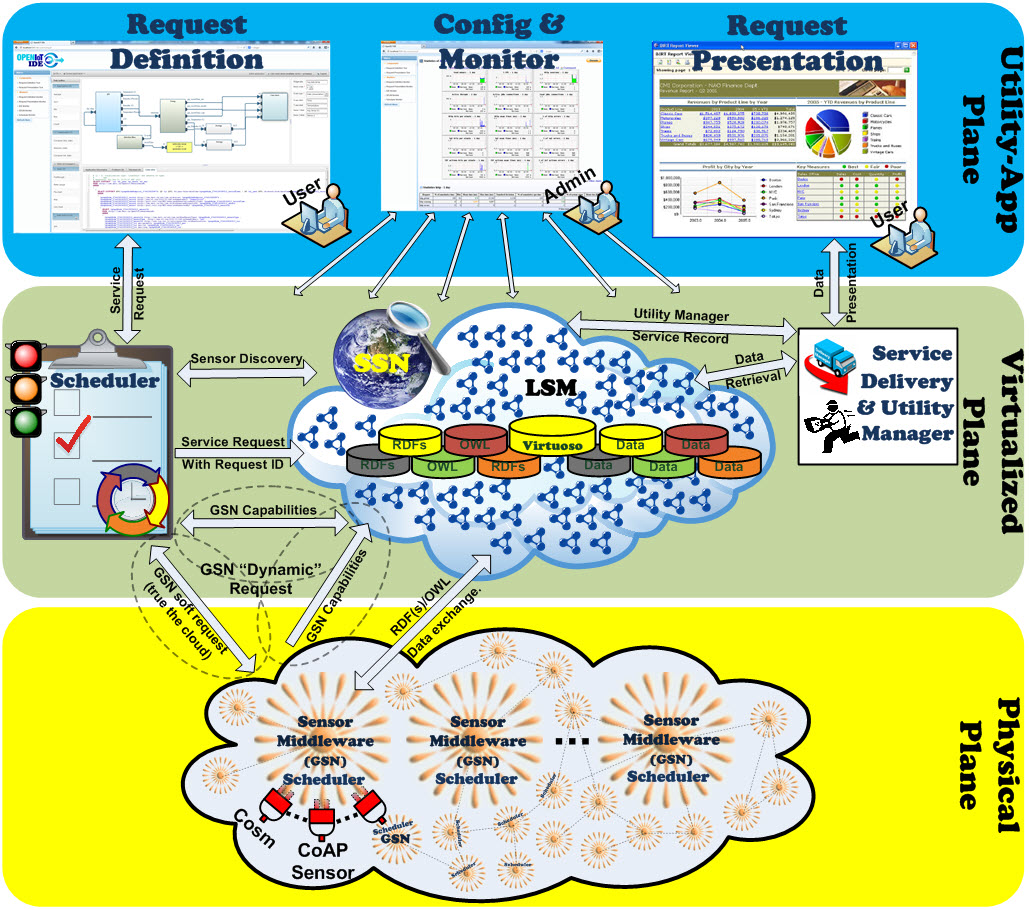
\includegraphics[width=1\linewidth]{Imagens/Cap_3/OpenIoT-Architecture}
\par\end{centering}
\caption{Arquitetura OpenIoT \cite{ZShelby2009} \label{fig:OpenIoT}}
\end{figure}


\paragraph*{Plano Utilitário / Aplicação }
\begin{itemize}
\item O componente \emph{Request Definition,} permite especificação, em
tempo de execução, de solicitações de serviços para a plataforma OpenIoT,
fornecendo uma interface Web 2.0. Compreende um conjunto de serviços
para a especificar e formular tais pedidos, ao mesmo tempo, submetê-los
ao agendador (\emph{Scheduler)} global.
\item O componente \emph{Request Presentation}, seleciona mashups a partir
de uma biblioteca apropriada, a fim de facilitar a apresentação de
um serviço em uma interface Web 2.0. Para visualizar estes serviços,
ele se comunica diretamente com o Service Delivery \& Utility Manager,
de modo a recuperar os dados relevantes.
\item A componente de configuração e monitoramento (\emph{Configuration
and Monitoring}), permite o gerenciamento e configuração de funcionalidades
sobre os sensores e os serviços que são implantados dentro da plataforma
OpenIoT. Além disso, permite ao usuário monitorar o estado dos diferentes
módulos implementados.
\end{itemize}

\paragraph*{Plano Virtualizado}
\begin{itemize}
\item O agendador (Scheduler) processa todas as solicitações de serviços
a partir da definição da solicitação (Request Definition) e garante
o seu acesso adequado aos recursos (por exemplo, fluxos de dados)
de que necessitam. 
\item A Nuvem de armazenamento de dados (LSM-Light), permite o armazenamento
de fluxos de dados provenientes do sensor, agindo assim como um banco
de dados em nuvem. O serviço armazena os metadados necessários para
o funcionamento da plataforma OpenIoT (dados funcionais). A implementação
do protótipo da plataforma OpenIoT usa o LSM Middleware, que foi re-projetado
com funcionalidades de dados push-pull e interfaces para permitir
streaming de processamento baseado em nuvem.
\item O serviço de entrega e gerenciador de utilitários (Service Delivery
\& Utility Manager), executa um duplo papel. Por um lado, ele combina
os fluxos de dados como indicado pelos fluxos de trabalho (workflows)
dentro do sistema OpenIoT a fim de entregar o serviço solicitado (com
a ajuda da consulta SPARQL fornecido pelo Scheduler), quer para a
solicitação de apresentação ou um aplicativo externo. Por outro lado,
esse componente atua como um mecanismo de medição de utilização dos
serviços, o que mantém o controle das métricas cada serviço individualmente.
\end{itemize}

\paragraph*{Plano Físico}
\begin{itemize}
\item O Sensor-Middleware (Extended Global Sensor Network, X-GSN), recolhe,
filtra, combina, e semanticamente anota fluxos de dados a partir de
sensores virtuais ou dispositivos físicos. Ele atua como um hub entre
a plataforma OpenIoT e o mundo físico. O Sensor-Middleware é implantado
com base em uma ou mais instâncias distribuídos (nós), que podem pertencer
a diferentes entidades administrativas. A implementação do protótipo
da plataforma OpenIoT usa o sensor-middleware GSN que foi ampliado
e chamado X-GSN.
\end{itemize}


\section{Eclipse IoT}

Eclipse IoT é um ecossistema de empresas e indivíduos que trabalham
em conjunto para estabelecer uma Internet das Coisas com base em tecnologias
abertas\cite{eclipse:iot}. O projeto fornece blocos de construção
que se apoiam em cima de padrões e protocolos abertos e fornecem serviços
e estruturas adicionais para gerenciamento de dispositivos, comunicação
e soluções verticais.

O primeiro projeto Eclipse IoT começou em novembro de 2012, hoje é
composto por subprojetos, focados no desenvolvimento de aplicações
para Internet das coisas e M2M. Em seguida é apresentado os principais
projetos mantidos de grupo.

\subsection{Padrões e Protocolos}
\begin{itemize}
\item \textbf{Paho}: prevê a implementação de clientes para o protocolo
de mensagens MQTT. O Paho, inclui clientes para Java, C, C++, Python,
JavaScript e outras implementações da da norma MQTT;
\item \textbf{Mosquitto}: implementação do servidor de MQTT;
\item \textbf{Californium}: é uma implementação Java do CoAP (Constrained
Application Protocol);
\item \textbf{OM2M}: é uma implementação do padrão OneM2M\cite{swetina2014toward}
(anteriormente chamado de padrão ETSI M2M). OM2M é um conjunto de
serviços Java e OSGi que implementam o padrão OneM2M;
\item \textbf{Wakaama}: é uma implementação do protocolo OMA Lightweight
M2M, para o dispositivos e gerenciamento de serviços. Wakaama é escrito
em C e projetado para ser portátil para sistemas compatíveis com POSIX.
\end{itemize}

\subsection{Frameworks e Serviços}
\begin{itemize}
\item \textbf{Kura}: é um conjunto de serviços Java e OSGi que implementam
os serviços comuns necessários para um gateway de Internet das Coisas,
tais como: (1) conexão de I/O com portas seriais, USB, Bluetooth,
GPS, (2) serviços de dados, (3) gerenciamento remoto, etc.
\item \textbf{Eclipse SCADA}: é um conjunto de serviços Java e OSGi para
a criação de sistemas de controle industrial que monitoram e controlam
processos industriais, como o chão de fábrica ou fazendas solares.
\item \textbf{Eclipse SmartHome}: é um conjunto de serviços para integração
de domótica em Java e OSGi. Este projeto fornece um ponto de acesso
uniforme para os diversos dispositivos e protocolos de automação residencial
diferentes.
\item \textbf{Ponte}: é um broker projetado para fazer a ponte entre protocolos
diferentes da Internet das Coisas (como MQTT e CoAP) e fornecer uma
API REST para esses padrões.
\item \textbf{Concierge}: é uma implementação do padrão OSGi, voltado para
pequenos dispositivos da Internet das Coisas.
\item \textbf{Krikkit}: é um projeto para definir regras para as mensagens
que passam através de um dispositivo de borda (edge device).
\item \textbf{Mihini}: é um framework baseado em Lua para a criação de aplicativos
para gateways IoT e M2M.
\end{itemize}
O Eclipse IoT é um projeto que vêm ganhando tração e incorporando
novos projetos\cite{eclipse:iot:projects}. Hoje conta com cerca de
110 colaboradores e é apoiados por empresas como IBM, Eurotech, 2lemetry,
Cisco, e outras.

\section{BUTLER}

BUTLER, acrônimo de uBiquitous, secUre inTernet-of-things with Location
and contExtawaReness, é um desenvolvido no âmbito do FP7, lançado
oficialmente em 2014, com o propósito de possibilitar o \textquotedbl{}desenvolvimento
de aplicações seguras e inteligentes de assistência pessoal graças
a um sistema pervasivo ciente de contexto e localização\textquotedbl{}\cite{BUTLER}.
BUTLER se concentra em:
\begin{itemize}
\item Melhorar / criar tecnologias para implementar uma Internet das Coisas
que seja segura (ligações seguras do físico para as camadas de aplicação),
pervasiva (aplicações abrangem diferentes cenários) e dependente do
contexto (ajusta às necessidades do usuário).
\item Integração / desenvolvimento de uma arquitetura em rede de dispositivos
inteligentes, onde os dispositivos podem ser categorizadas como SmartObjects
(sensores, atuadores, gateways), Smart Mobile (dispositivo pessoal
de usuário) e SmartServers (fornecedores de conteúdos e serviços).
\item Realização de estudos de caso para mostrar e ajudar a melhorar o projeto.
\end{itemize}
Foram definidos papéis de segurança no nível de aplicação, que refletem
os stakeholders participantes das interações em cada cenário. Os papéis
definidos no projeto são\cite{BUTLER:tec}:
\begin{itemize}
\item Usuário: entidade que ganha acesso a um recurso. Normalmente é um
humano, mas pode ser também uma aplicação;
\item Provedor de Recurso: entidade que provê um recurso e opcionalmente
o atualiza. Ele deve conferir o token de acesso apresentado para que
possa prover/atualizar um recurso;
\item Consumidor de Recurso: aplicação cliente recuperando e consumindo
recursos;
\item Servidor de Autorização: é a entidade que implementa a gestão de controle
de acesso. É responsável pela autenticação do usuário e autorização
do consumidor de recurso através da geração de um token de acesso,
relacionado ao recurso que se deseja acessar. Opcionalmente, pode
delegar a tarefa de autenticação para o servidor de autenticação;
\item Servidor de Autenticação: esta entidade pode ser utilizada pelo servidor
de autorização de modo a confiar em um protocolo de autenticação que
não é implementado nativamente no servidor de autorização. Isso significa
que o servidor de autenticação e o servidor de autorização precisarão
fazer a federação de identidades de usuários.
\end{itemize}
A arquitetura do projeto é baseada nas arquiteturas IoT-A e FI-WARE.
A figura \ref{fig:BUTLER}, apresenta as quatro principais camadas
definidas na arquitetura. 

\begin{figure}
\begin{centering}
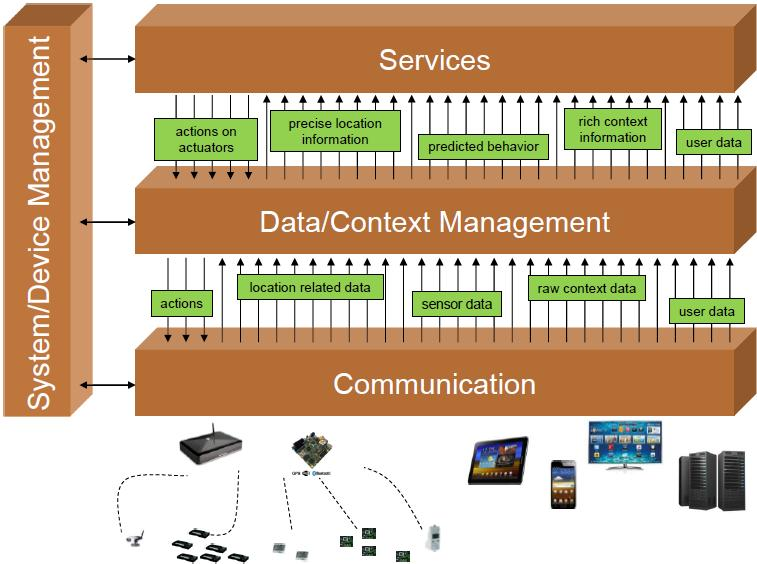
\includegraphics[width=1\linewidth]{Imagens/Cap_3/butler}
\par\end{centering}
\caption{Arquitetura proposta por BUTLER \cite{BUTLER}\label{fig:BUTLER}}
\end{figure}

\begin{itemize}
\item \textbf{Communications Layer:} lida com a infraestrutura de comunicação
fim-a-fim (com base em normas, tanto quanto possível), conectando
objetos inteligentes (SmartObjects), dispositivos móveis (SmartMobiles)
e plataformas de serviços (SmartObject Gateways e SmartServers). 
\item \textbf{Data/Context Management Layer}: especifica modelos de dados,
interfaces e procedimentos de coleta e processamento de dados. Com
informações de contexto, transforma os dados brutos em informações
ricas. 
\item \textbf{Services Layer}: define componentes e interfaces para a descrição,
descoberta, implantação e provisionamento de serviços sensíveis ao
contexto. 
\item \textbf{System/Device Management Layer:} gerencia e mantém objetos
inteligentes, serviços e outras entidades, como a configuração, gerenciamento
de desempenho, ou diagnósticos.
\end{itemize}

\section{LinkSmart (HYDRA)}

O LinkSmart (anteriormente chamado Hydra), tem como objetivo desenvolver
um middleware para sistemas embarcados inteligentes, baseado em uma
arquitetura orientada a serviços, implementável em redes novas ou
existentes, com ou sem fio, de dispositivos heterogêneos que operam
com recursos limitados em termos de energia, poder de computação e
uso da memória\cite{sarnovsky2007hydra}. A arquitetura LinkSmart
é baseada em três camadas: a camada física, a camada de middleware,
e a camada de aplicação. O middleware HYDRA, foi testado em três domínios,
tais como automação predial, área da saúde, e agricultura \cite{jahn2010energy}).
O usuário pode acessar os serviços oferecidos pelo HYDRA através de
uma interface inteligente móvel.

Middleware LinkSmart é um software inteligente que é colocado entre
as aplicações e o sistema operacional para lidar com várias tarefas
de uma forma eficiente em termos de custos. Este middleware fornece
uma interface de serviço web para interagir com todos os dispositivos
físicos, atuadores, sensores ou subsistemas, independentemente de
suas tecnologias de interface de rede, por exemplo, Bluetooth, RF,
ZigBee, RFID, Wi-Fi, etc.

Este middleware foi projetado para facilitar a interação com dispositivos,
abstraindo a partir das informações detalhadas sobre esses dispositivos
e suas redes. O LinkSmart considera cada dispositivo como um serviço,
e usa linguagens de ontologias, por exemplo, OWL, OWL-s e SAWSDL,
para definir as descrições semânticas desses dispositivos. Além disso,
ele fornece uma camada de serviço inteligente, que permite aos usuários
finais interagirem com esses dispositivos, sem lidar com a tecnologia
de comunicação que é suportado pelos dispositivos.


\section{TinyDB}

O middleware TinyDB\cite{madden2005tinydb} foi um dos primeiros projetos
a propor a ideia de abstração dispositivos. O TinyDB permite que usuários
finais interajam com os dispositivos sem saber sobre o detalhes da
especificação dispositivos, tais como os protocolos de comunicação
que são suportado por esses dispositivos.

O projeto fornece uma linguagem de domínio específico (DSL) para usuários
finais interagirem com os dispositivos. Sua DSL é uma linguagem de
consulta que suporta seleção, junção, projeção, e agregação, para
trabalhar com um ambiente de sensoriamento embarcado. Esta DSL permite
que um usuário final obtenha informações sobre o tempo, lugar, tipo
e método de amostragem em um ambiente de sensoriamento embarcado.
TinyDB suporta os seguintes tipos de consultas:
\begin{itemize}
\item Monitoring Queries: Ela pede o valor de um ou mais atributos periodicamente
e continuamente, tais como, informações sobre a temperatura.
\item Network Health Queries: Ele fornece informações sobre a própria rede.
Por exemplo, a seleção de nós vizinhos, com baixa vida útil de bateria.
\item Exploratory Query: Ela mostra o estado de um nó específico ou de um
conjunto de nós em um momento específico, tais como, por exemplo,
selecionar a temperatura do sensor através da sua identificação.
\item Actuation Query: Este tipo de consulta pode ser usada para pedir uma
ação física. Por exemplo, um usuário final pode querer ligar um ventilador
num ambiente em que a temperatura é superior a um limiar. 
\end{itemize}

\section{IoT@Work}

Este projeto é focado na automação industrial, levando em considerações
requisitos de comunicação e segurança. O projeto foi fundado pelo
FP7 e é liderado pelo Siemens AG\cite{IoTWork:site}\cite{rotondi2011project}.

O projeto tem como objetivo reduzir custos operacionais na configuração,
comissionamento, e manutenção da fabricação, principalmente diminuindo
o tempo para adaptação a mudanças no sistema.

Com base nos resultados dos projetos de investigação realizados, o
IoT@Work se concentra em melhorar a infraestrutura de comunicação
e middleware para construir a auto-gestão e redes resilientes e arquiteturas
de aplicativos orientados a serviços adaptados para ambientes de fábrica.

Os principais objetivos técnicos do projeto estão centrados em torno
dos seguintes objetivos:
\begin{itemize}
\item A dissociação entre a aplicação de automação e a configuração de rede
e operação, a fim de:

\begin{itemize}
\item Fornecer serviços avançados de comunicações que atendem demandas da
aplicação em termos de confiabilidade, comunicação em tempo real,
escalabilidade e segurança.
\item Reduzir os efeitos do processo de reconfiguração da aplicação sobre
o montante do planejamento manual necessária a nível da rede; 
\end{itemize}
\item Integrar mais auto-gestão em uma rede ``Plug\&Work'', a fim de:

\begin{itemize}
\item Ativar ``Plug\&Work'' em todos os níveis, especialmente durante
a fase de configuração das redes de automação industrial;
\item Levar em conta a semântica da aplicação e os fluxos de trabalho na
estruturação e otimização da operação da rede.
\end{itemize}
\item Garantir a resiliência e segurança em sistemas de automação em execução,
a fim de:

\begin{itemize}
\item Suporte a cenários de fabricação adaptáveis e ágeis, ao mesmo tempo
garantir e proteger a confiabilidade e a resiliência dos sistemas;
\item Integrar mecanismos de segurança fortes a nível arquitetônico e evitar
acesso não autorizado e interferências indesejadas com o processo
de produção.
\end{itemize}
\end{itemize}

\subsection{Arquitetura}

A arquitetura para este projeto foi desenvolvido em cooperação com
IoT-A\cite{rotondi2011project} e consiste de várias funções que são
implementadas por vários componentes, que são agrupados três camadas
principais, confirme a Figura \ref{fig:iot_work}.

\begin{figure}
\begin{centering}
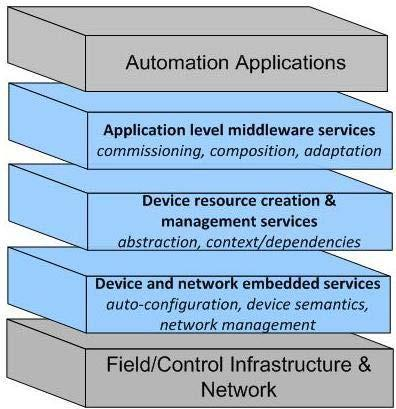
\includegraphics[width=0.5\linewidth]{Imagens/Cap_3/iot_work}
\par\end{centering}
\caption{Arquitetura IOT@Work - Camadas funcionais \cite{rotondi2011project}\label{fig:iot_work}}
\end{figure}

\textbf{Device and network embedded services}: realizar funções de
gestão, como a atribuição de identificadores, coletando semântica
de dispositivos e contexto e gestão de interfaces de comunicação.

\textbf{Device resource creation \& management services}: executar
agregação e gestão dos recursos e serviços incorporados e funções,
tais como o fornecimento de serviços de diretórios, abstração de redes
e monitoramento do sistema de baixo nível e de gestão de segurança.

\textbf{Application level middleware services}: oferece suporte para
aplicação por meio de serviços de middleware específicos para cenários
da Internet das Coisas. Nesta camada, a lógica do aplicativo é interpretada
através de configuração ou em tempo de execução e definição das interfaces
com os diferentes componentes IoT .

\subsection{Tecnologias Integradas}

Descrição da principais tecnologias envolvidas na construção da arquitetura
do IoT@Work\cite{IoTWork:site}.
\begin{itemize}
\item \textbf{Serviço de Diretório}: fornece um acesso unificado e baseado
em padrões para acesso às informações, escondendo a complexidade e
variedade de protocolos e formatos. Armazena informações que podem
ser atualizadas através da API RESTful.
\item \textbf{Auto-configuração de rede Ethernet em tempo real}: Atribuição
de endereço IP e URL, descoberta, e configuração em tempo real.
\item \textbf{Gerenciamento de Eventos (Serviço de Notificação de Evento}):
é um componente de middleware que atua como um conector flexível e
escalável entre fontes de eventos (ex.: \emph{Publishers}) e consumidores
de eventos (ex.: \emph{Subscribers}).
\item \textbf{Controle de Acesso}: O controle de acesso é apresentado em
dois níveis: (1) controle de acesso granular para as coisas, agentes,
aplicações, consumidores de dados, em todos os níveis e (2) controle
de acesso para garantir a confiabilidade da comunicação e estado da
configuração aos dispositivos embarcados.
\item \textbf{Processamento de Eventos Complexos (CEP)}: realiza processamento
inteligente de mensagem (análise de falhas, manutenção preditiva),
suporta a auto-gestão e permite a filtragem e combinação de eventos
para criar uma nova funcionalidade (usando regras inteligentes).
\item \textbf{Particionamento de Rede}: Ferramenta de gerenciamento de virtualização
de rede.
\end{itemize}

\section{Plataformas Comerciais}

O grande potencial esperado para Internet das Coisas\cite{GoldmanSachs2014,url:cisco:iot:2015,url:webintel:2015},
tem despertado a atenção de grandes empresas, que vem expandindo seus
serviços, muitos deles baseados em nuvem, para atender requisitos
de projetos de Internet das Coisas. A seguir, é apresentada uma lista
resumida das principais empresas de oferecem serviços para IoT.

\subsection{Google}

A Google vem investindo no cenário de IoT, e expandindo sua plataforma
em nuvem, \emph{Google Cloud Platform}, para atender os requisitos
de IoT. Os principais serviços incorporados na sua plataforma, são
destacados a seguir:
\begin{itemize}
\item Google Cloud Pub/Sub: É projetado para fornecer de mensagens assíncronas
muitos-para-muitos de maneira confiável entre aplicações.
\item Device Streaming: Oferece suporte para processamento, armazenamento
e análise de centenas de milhões de eventos.
\end{itemize}
A aquisição da empresa Nest em fevereiro de 2014, por cerca de 3,2
bilhões de dólares, vem mostrando o direcionamento da empresa para
áreas de computação embarcada e IoT. Outro projeto em desenvolvimento
é o Brillo, que tem como objetivo fornecer um sistema operacional
para dispositivos embarcados baseados em plataformas ARM, Intel x86,
and MIPS, focado em dispositivos com memória RAM a partir de 32MB.


\subsection{Oracle}

Oferece uma plataforma\cite{oracle:iot} baseada em nuvem, para conectar,
analisar, e integrar dispositivos, processos de negócios e aplicações.
As principais recursos oferecidos estão relacionados à virtualização
de dispositivos, comunicação bi-direcional, gerenciamento de metadados,
processamento de eventos e \emph{Big Data}. 

\subsection{Salesforce - IoT Cloud}

A plataforma oferecida pela Salesforce\cite{salesforce:iot}, é um
serviço baseado em nuvem, focado principalmente em processamento de
eventos complexos integrados com processos de negócio. O projeto denominado
Salesforce Thunder, é a peça central da plataforma, e é apresentado
pela empresa, como o motor de processamento de eventos mais rápido.

\subsection{IBM}

A plataforma ``IBM IoT Foundation''\cite{ibm:iot}, permite que
as organizações conectem dispositivos de forma fácil e segura, a partir
de chips à dispositivos inteligentes. Escalando através de serviços
baseados em nuvem, e usando análises ricas, a plataforma fornece às
organizações uma nova visão de inovação e transformação.

Outro projeto liderado pela empresa é o ``Watson Internet of Things'',
que tem o foco na inteligência computacional de cognição e inferência.

\subsection{Amazon IoT}

O AWS IoT\cite{amazom:iot} é uma plataforma que permite conectar
dispositivos aos serviços da AWS e a outros serviços. Permite interação,
processamento dos dados dos dispositivos e integração com aplicações,
mesmo quando eles estiverem off-line. A empresa oferece um SDK (AWS
IoT Device SDK), que permite que os dispositivos facilmente se conectem
à nuvem usando protocolos MQTT ou HTTP, suportando dispositivos como
Arduino e linguagens C e JavaScript.

\subsection{Microsoft}

A recente parceria entre Microsoft e Arduino\cite{microsoft:arduino},
demostra a aproximação da empresa na construção de projetos de IoT
e o apoio à projetos open source. A empresa possui projetos tanto
a área de sistemas embarcados, com o sistema operacional Windows 10
IoT Core, compatível com Raspberry Pi, quando para serviços em nuvem,
com o Azure IoT Suite\cite{microsoft:iot}.

\subsection{Intel}

A Intel é outra empresa que vem apostando fortemente no mercado de
IoT, contando com projetos para dispositivos embarcados e soluções
em nuvem. Na perspectiva de projetos cloud a empresa oferece o ``Intel\textregistered{}
IoT Platform''\cite{intel:iot}, com o objetivo de interconectar
dispositivos de forma segura e escalável, permitindo a análise e extração
de valor dos dados.

Na área de dispositivos embarcados a empresa oferece kits de desenvolvimento
que contam com a placa Galileo, com compatível e certificada pelo
Arduino\footnote{https://www.arduino.cc/en/ArduinoCertified/IntelGalileo},
e a placa Intel\textregistered{} Edison\footnote{https://software.intel.com/pt-br/iot/hardware/edison},
também compatível com Arduino e de fácil integração aos serviços Microsoft
Azure IoT Suite e Amazon AWS.

\subsection{Xynvely}

A plataforma Xively\cite{Xively:iot}, desenvolvida pela empresa LogMeIn,
utiliza serviços de nuvem para gerenciar dados providos por dispositivos.
A plataforma fornece uma API para envio de dados a partir dos sensores,
permitindo assim a visualização de dados históricos e provendo mecanismos
para disparar eventos com base nos dados gerados pelos sensores (os
chamados triggers). Na plataforma, os dados são organizados em feeds,
datapoints e datastreams.

\section{Considerações Finais}

\subsection{Análise das Plataformas Abertas}

Os projetos selecionados para análise tem como característica em comum
as capacidades de abstração de hardware, código fonte disponível,
e o fato de terem sido desenvolvidos recentemente. O TinyDB e as plataformas
comerciais não serão incluídos nessa análise.
\begin{itemize}
\item Disponibilidade de documentação e código fonte: 

\begin{itemize}
\item O(s) projeto(s): BUTLER, IoT@Work e LinkSmart, são projetos que apesar
de terem código fonte disponível, não possuem informações de como
realizar o processo de compilação, ou mesmo, não é disponibilizado
o código de todos os componentes, impossibilitando a análise e testes
aprofundados.
\item O(s) projeto(s): OpenIoT e Eclipse IoT, possuem boa quantidade de
documentação, guias de instalação e o código de todos componentes
são acessíveis (github). Porém os dois possuem um processo de ``setup''
relativamente complexo.
\end{itemize}
\item Abstração do Hardware:

\begin{itemize}
\item Todos os projetos avaliados atendem bem a este requisito. No Eclipse
IoT ele é implementado pelo sub-projeto chamado Leshan\footnote{http://www.eclipse.org/leshan/},
focado na comunicação M2M e CoAP.
\end{itemize}
\item Integração com plataformas de hardware mencionadas na seção \ref{sec:Plataformas-de-Desenvolvimento}:

\begin{itemize}
\item O(s) projeto(s): Eclipse IoT, é um dos poucos a dar ênfase nessas
plataformas, porém, devido o requisito anterior, existem algumas lacunas
a serem abordadas. 
\end{itemize}
\item Complexidade no desenvolvimento de projetos:

\begin{itemize}
\item O(s) projeto(s): BUTLER, IoT@Work e LinkSmart, não puderam ser avaliados
conforme a complexidade do desenvolvimento, pois não possuem instaladores,
nem foi possível a compilação a partir dos códigos fonte.
\item O(s) projeto(s): Eclipse IoT e OpenIoT, devido à grande quantidade
de componentes, possuem um processo de compilação complexo e demoraram
para serem configurados. O Eclipse IoT é o mais favorável neste quesito,
apesar de termos encontrado algumas falhas nos testes iniciais.
\end{itemize}
\item Ferramentas para auxílio na construção das aplicações embarcadas (firmware):

\begin{itemize}
\item O(s) projeto(s): Eclipse IoT, possui subprojetos WAKAAMA e Leshan,
que possuem recursos e bibliotecas em C para desenvolvimento para
microcontroladores, porém o mesmo, necessita de 100kb de flash e 10kb
de RAM. O sub-projeto Eclipse Paho, disponibiliza bibliotecas compatíveis
com o Arduino para comunicação usando MQTT.
\end{itemize}
\item Ferramentas de visualização e interface com os dispositivos:

\begin{itemize}
\item O(s) projeto(s): OpenIoT, oferece interfaces avançadas para configuração
de dispositivos, composição e orquestração de serviços. O projeto
Eclipse IoT, mais especificamente o sub-projeto Leshan, possuí alguns
recursos simples para interação com os dispositivos.
\end{itemize}
\item Abstração de comunicações: Bluetooth, USB, Ethernet, WiFi:

\begin{itemize}
\item A maioria dos projetos estão voltados para comunicação usando protocolo
IP, com exceção do Eclipse IoT (subprojeto Kura), que possui implementações
para comunicação USB e Bluetooth.
\end{itemize}
\item Auxílio na construção de aplicações Web:

\begin{itemize}
\item O(s) projeto(s): Eclipse IoT, possuem implementações de clientes MQTT
em JavaScript no sub-projeto Paho, porém não possui nenhuma implementação
para abstração de dispositivos na camada Web em JavaScript. 
\end{itemize}
\item Auxílio na construção de aplicações Mobile (Android):

\begin{itemize}
\item O(s) projeto(s): Eclipse IoT, possui apenas implementação para clientes
MQTT, e no projeto OpenIoT, foram encontradas apenas interfaces gráficas
de visualização de dispositivos, nenhuma ferramenta específica para
desenvolvimento.
\end{itemize}
\end{itemize}


\subsection{Análise das Plataformas Comerciais}

Não é objetivo desta dissertação o aprofundamento na análise de plataformas
proprietárias, limitando-se apenas a algumas considerações.

As plataformas proprietárias oferecem um requisito importante para
projetos de IoT, principalmente, quando os mesmos necessitarem trabalhar
com uma grande quantidade de dispositivos, que está relacionado à
escalabilidade. A maioria das soluções abordadas neste trabalho, são
de empresas que oferecem outros serviços relacionados a \emph{cloud
computing}, que por natureza, necessitam de um infraestrutura altamente
escalável. Por outro lado, essas plataformas comerciais precisam estar
baseadas em protocolos abertos para sua ampla difusão e penetração
do mercado de IoT.

As empresas que mais se destacam no desenvolvimento e apoio de padrões
abertos são a Amazon AWS, Microsoft (contrariando as expectativas)
e Intel. Estas empresas, também oferecem suporte para os hardwares
abertos (como Arduino), e biliotecas para a integração com seus serviços
em núvem.

A Google, na sua plataforma, parece estar direcionada a usar seus
próprios padrões\footnote{http://venturebeat.com/2015/05/28/google-announces-brillo-os-for-the-internet-of-things/}\footnote{https://cloud.google.com/pubsub/docs},
e até o momento não oferece suporte ao MQTT. 
